%%
% CS 4510 Homework LaTex Template
% (C) Copyright Junghyun Kim(conankun@gatech.edu)
%%
%Preset
\documentclass[10pt, legalpaper]{exam}
\usepackage[utf8]{inputenc}
\usepackage[margin=.75in]{geometry}
\usepackage{amsmath,amssymb}
\usepackage{multicol}
\usepackage{graphicx}
\usepackage{tikz}
\usepackage{pgf}
\usetikzlibrary{arrows,automata}
\usepackage{enumerate}

% Configuración del Encabezado
\newcommand{\class}{CS 4510: Automata and Complexity}
\newcommand{\term}{Fall 2017}
\newcommand{\examnum}{Homework 1}
\newcommand{\examdate}{Due: Sep. 11th. 2017}
\pagestyle{head}
\runningheader{\class}{\examnum\ - Page \thepage\ of \numpages}{\examdate}
\runningheadrule

% Configuración de la tabla de calificación
\pointpoints{punto}{Points}
\hpword{Points:}
\vpword{Points}
\vtword{Total:}
\htword{Total}
\vsword{Score}
\hsword{Score:}
\vqword{Problem}
\hqword{Question:}

\begin{document}
% Definición del Encabezado
\noindent
\begin{tabular*}{\textwidth}{l @{\extracolsep{\fill}} r @{\extracolsep{6pt}} l}
\textbf{\class} &  & \\
\textbf{\term} &&\\
\textbf{\examnum} & \textbf{Name:} & \makebox[2.5in]{\hrulefill}\\
\textbf{\examdate} &&\\
\end{tabular*}\\
\rule[2ex]{\textwidth}{2pt}

% Bloque de instrucciones
\noindent
This assignment contains \numpages\; pages (including this cover page) and \numquestions\; questions. Print  your name at the top of this page, and put your initials on the top of every other page, in case the pages become separated. \\\\
Please show your work on each problem. You might get partial credit for your work. Also, \textbf{do not write in the table below}.

% Tabla de calificaciones
\begin{center}
\textbf{Table for Instructor use only}. \\
\addpoints
% Puede presentar la tabla de calificación en orientación vertical [v] u horizontal [h]
\gradetable[h][questions]
\end{center}

\noindent
\rule[2ex]{\textwidth}{2pt}

% Questions.
\begin{questions}
\newpage
\addpoints
\question[25] Give state diagrams of DFAs recognizing the follwing languages. In all parts, the alphabet is $\{0, 1\}$.
\begin{enumerate}[(a)]
\item $\{w| w \textrm{ contains at least three 1s}\}$
\item $\{w| w \textrm{ starts with 0 and has odd length, or starts with 1 and has even length}\}$
\item $\{w| w \textrm{ doesn't contain the substring 110}\}$
\item $\{w| w \textrm{ is any string except 11 and 111}\}$
\item $\{w| w \textrm{ contains an even number of 0s, or contains exactly two 1s}\}$
\end{enumerate}

\subsection*{Answers}

\begin{enumerate}[(a)]
    \setlength\itemsep{5em}

    \item 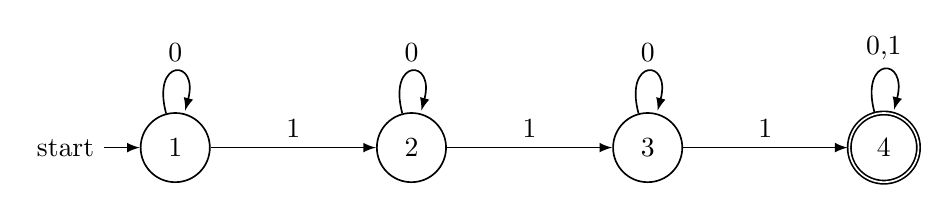
\begin{tikzpicture}[->,
            >=latex,
            auto,
            node distance=3cm,
            semithick,
            baseline=(top.base)]
            
        \node[initial,state]   (1)              {$1$};
        \node[state]           (2) [right of=1] {$2$};
        \node[state]           (3) [right of=2] {$3$};
        \node[accepting,state] (4) [right of=3] {$4$};

        \path (1) edge [loop above] node (top) {0}   (1)
                  edge              node       {1}   (2)
              (2) edge [loop above] node       {0}   (2)
                  edge              node       {1}   (3)
              (3) edge [loop above] node       {0}   (3)
                  edge              node       {1}   (4)
              (4) edge [loop above] node       {0,1} (4);
                  
    \end{tikzpicture}
           
    \item 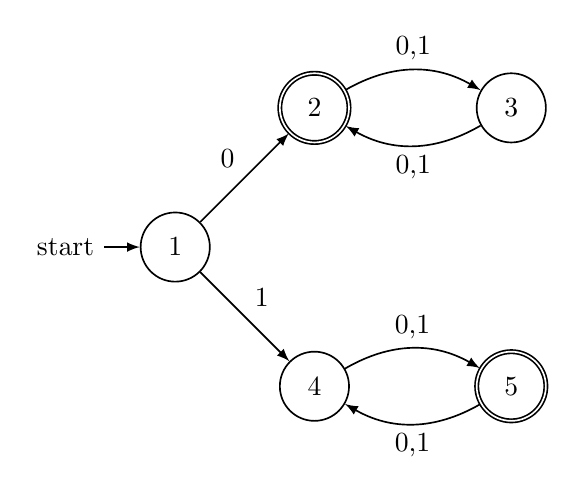
\begin{tikzpicture}[->,
            >=latex,
            auto,
            node distance=2.5cm,
            semithick,
            baseline=(top.base)]

        \node[initial,state]   (1)                    {$1$};
        \node[accepting,state] (2) [above right of=1] {$2$};
        \node[state]           (3) [right of=2]       {$3$};
        \node[state]           (4) [below right of=1] {$4$};
        \node[accepting,state] (5) [right of=4]       {$5$};

        \path (1) edge             node       {0}   (2)
                  edge             node       {1}   (4)
              (2) edge [bend left] node (top) {0,1} (3)
              (3) edge [bend left] node       {0,1} (2)
              (4) edge [bend left] node       {0,1} (5)
              (5) edge [bend left] node       {0,1} (4);

    \end{tikzpicture}
    
    \item 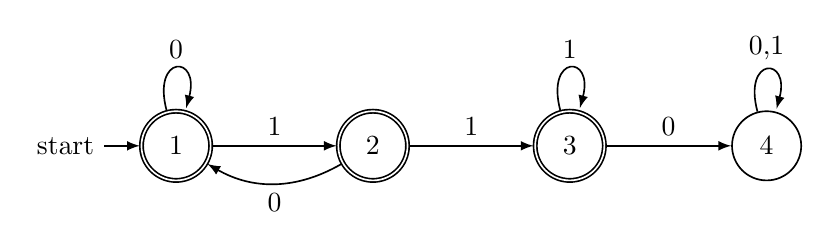
\begin{tikzpicture}[->,
            >=latex,
            auto,
            node distance=2.5cm,
            semithick,
            baseline=(top.base)]

        \node[initial,accepting,state] (1)              {$1$};
        \node[accepting,state]         (2) [right of=1] {$2$};
        \node[accepting,state]         (3) [right of=2] {$3$};
        \node[state]                   (4) [right of=3] {$4$};

        \path (1) edge [loop above] node (top) {0}   (1)
                  edge              node       {1}   (2)
              (2) edge [bend left]  node       {0}   (1)
                  edge              node       {1}   (3)
              (3) edge [loop above] node       {1}   (3)
                  edge              node       {0}   (4)
              (4) edge [loop above] node       {0,1} (4);

    \end{tikzpicture}
    
    \item 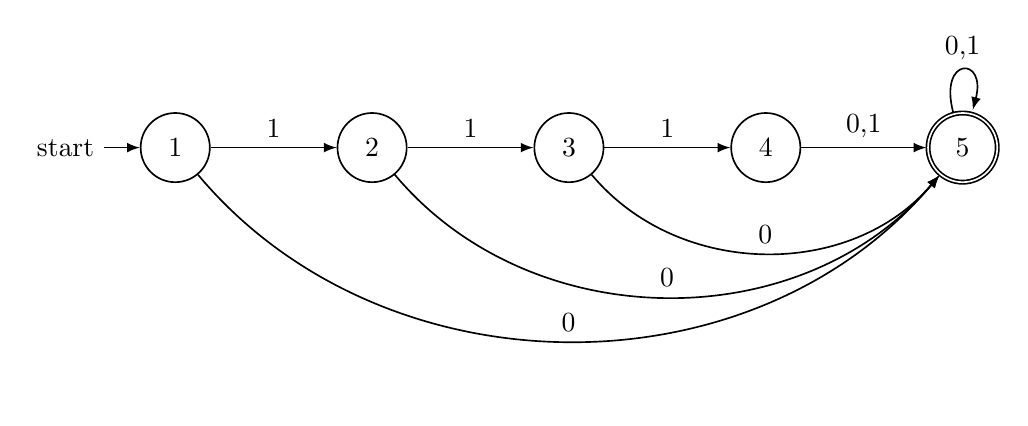
\begin{tikzpicture}[->,
            >=latex,
            auto,
            node distance=2.5cm,
            semithick,
            baseline=(top.base)]

        \node[initial,state]   (1)              {$1$};
        \node[state]           (2) [right of=1] {$2$};
        \node[state]           (3) [right of=2] {$3$};
        \node[state]           (4) [right of=3] {$4$};
        \node[accepting,state] (5) [right of=4] {$5$};

        \path (1) edge [bend right=50] node       {0}   (5)
                  edge                 node       {1}   (2)
              (2) edge [bend right=50] node       {0}   (5)
                  edge                 node       {1}   (3)
              (3) edge [bend right=50] node       {0}   (5)
                  edge                 node       {1}   (4)
              (4) edge                 node       {0,1} (5)
              (5) edge [loop above]    node (top) {0,1} (5);

    \end{tikzpicture}
    
    \item 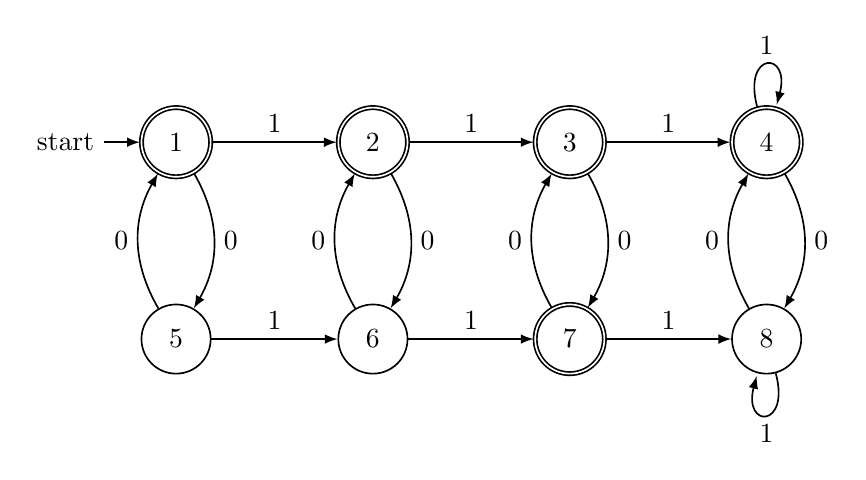
\begin{tikzpicture}[->,
            >=latex,
            auto,
            node distance=2.5cm,
            semithick,
            baseline=(top.base)]

        \node[initial,accepting,state] (1)               {$1$};
        \node[accepting,state]         (2)  [right of=1] {$2$};
        \node[accepting,state]         (3)  [right of=2] {$3$};
        \node[accepting,state]         (4)  [right of=3] {$4$};
        \node[state]                   (5)  [below of=1] {$5$};
        \node[state]                   (6)  [right of=5] {$6$};
        \node[accepting,state]         (7)  [right of=6] {$7$};        
        \node[state]                   (8)  [right of=7] {$8$};
        
        \path (1) edge [bend left]  node       {0} (5)
                  edge              node       {1} (2)
              (2) edge [bend left]  node       {0} (6)
                  edge              node       {1} (3)
              (3) edge [bend left]  node       {0} (7)
                  edge              node       {1} (4)
              (4) edge [bend left]  node       {0} (8)
                  edge [loop above] node (top) {1} (4)
              (5) edge [bend left]  node       {0} (1)
                  edge              node       {1} (6)
              (6) edge [bend left]  node       {0} (2)
                  edge              node       {1} (7)
              (7) edge [bend left]  node       {0} (3)
                  edge              node       {1} (8)
              (8) edge [bend left]  node       {0} (4)
                  edge [loop below] node       {1} (8);

    \end{tikzpicture}
\end{enumerate}

\newpage
\addpoints
\question[15] Give state diagram of NFAs with the specified number of states recognizing each of the following languages. In all parts, the alphabet is $\{0,1\}$
\begin{enumerate}[(a)]
\item {$\{w| w \textrm{ contains the substring 0101 (i.e., } w = x0101y \textrm{ for some } x \textrm{ and } y \textrm{)}\}$}
\item $\{w| w \textrm{ contains an even number of 0s, or contains exactly two 1s}\}$
\item {The language $0^{*}1^{*}0^{+}$ with three states}
\end{enumerate}

\subsection*{Answers}

\begin{enumerate}[(a)]
    \setlength\itemsep{5em}
    
    \item 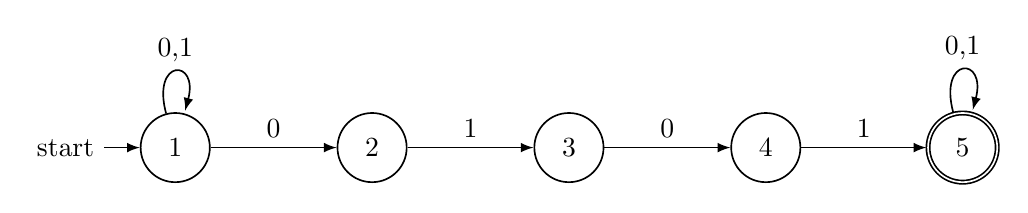
\begin{tikzpicture}[->,
            >=latex,
            auto,
            node distance=2.5cm,
            semithick,
            baseline=(top.base)]

        \node[initial,state]   (1)              {$1$};
        \node[state]           (2) [right of=1] {$2$};
        \node[state]           (3) [right of=2] {$3$};
        \node[state]           (4) [right of=3] {$4$};
        \node[accepting,state] (5) [right of=4] {$5$};

        \path (1) edge [loop above]         node (top) {0,1} (1)
                  edge                      node       {0}   (2)
              (2) edge                      node       {1}   (3)
              (3) edge                      node       {0}   (4)
              (4) edge                      node       {1}   (5)
              (5) edge [loop above]         node       {0,1} (5);

    \end{tikzpicture}

    \item 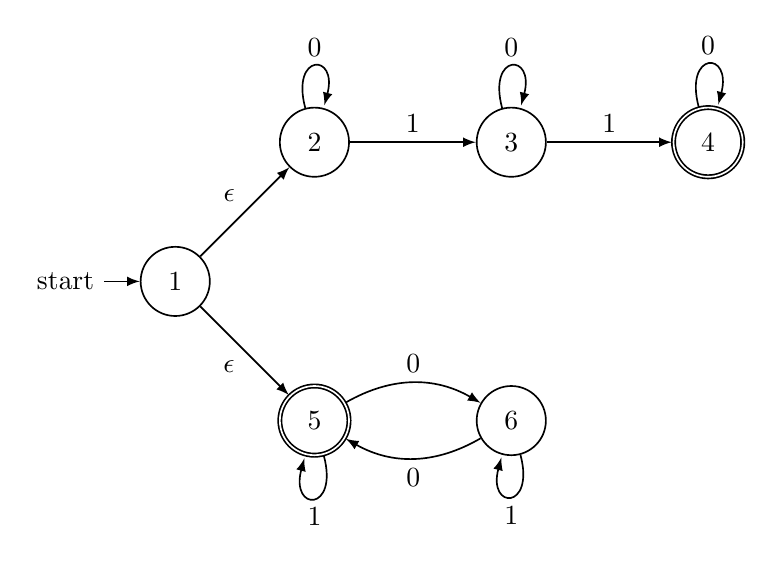
\begin{tikzpicture}[->,
            >=latex,
            auto,
            node distance=2.5cm,
            semithick,
            baseline=(top.base)]

        \node[initial,state]   (1)                    {$1$};
        \node[state]           (2) [above right of=1] {$2$};
        \node[state]           (3) [right of=2]       {$3$};
        \node[accepting,state] (4) [right of=3]       {$4$};
        \node[accepting,state] (5) [below right of=1] {$5$};
        \node[state]           (6) [right of=5]       {$6$};

        \path (1) edge              node       {$\epsilon$} (2)
                  edge [swap]       node       {$\epsilon$} (5)
              (2) edge [loop above] node (top) {0}          (2)
                  edge              node       {1}          (3)
              (3) edge [loop above] node       {0}          (3)
                  edge              node       {1}          (4)
              (4) edge [loop above] node       {0}          (4)
              (5) edge [loop below] node       {1}          (5)
                  edge [bend left]  node       {0}          (6)
              (6) edge [loop below] node       {1}          (6)
                  edge [bend left]  node       {0}          (5);
              
    \end{tikzpicture}
    
    \item 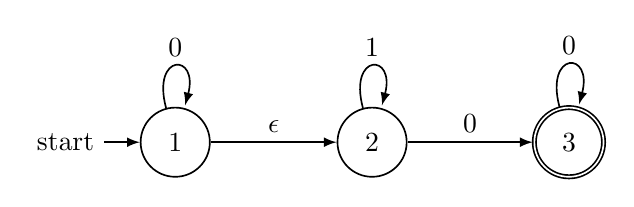
\begin{tikzpicture}[->,
            >=latex,
            auto,
            node distance=2.5cm,
            semithick,
            baseline=(top.base)]

        \node[initial,state]   (1)              {$1$};
        \node[state]           (2) [right of=1] {$2$};
        \node[accepting,state] (3) [right of=2] {$3$};

        \path (1) edge [loop above] node (top) {0}          (1)
                  edge              node       {$\epsilon$} (2)
              (2) edge [loop above] node       {1}          (2)
                  edge              node       {0}          (3)
              (3) edge [loop above] node       {0}          (3);
              
    \end{tikzpicture}    
\end{enumerate}

\newpage
\addpoints
\question[20] Please complete following proofs.
\begin{enumerate}[(a)]
\item {Show that if $M$ is a DFA that recognizes language $B$, swapping the accept and nonaccept states in $M$ yields a new DFA recognizing the complement of $B$. Conclude that the class of regular languages is closed under complement.}
\item {Show by giving an example that if $M$ is an NFA that recognizes language $C$, swapping the accept and nonaccept states in $M$ doesn't necessarily yield a new NFA that recognizes the complement of $C$. Is the class of languages recognized by NFAs closed under complement? Explain your answer.}
\end{enumerate}

\subsection*{Answers}

\begin{enumerate}[(a)]
    \item Let \(M_{1}\) be the DFA with swapped accept/nonaccept states and let \(B_{1}\) be the language recognized by \(M_{1}\). Consider an arbitrary string \(w\). If \(w \in B\), then it must be true that \(w \notin B_{1}\), since whichever accept state of \(M\) it ends on must be a nonaccept state of \(M_{1}\). If \(w \notin B\), then it must have ended on a nonaccept state of \(M\), which would be an accept state of \(M_{1}\). In this case \(w \in B_{1}\). Therefore \(B_{1}=\{w|w \notin B\}\). This is the definition of the complement of a set, so \(B_{1}=B^{\complement}\). \(B\) is a regular language because it is recognized by a DFA, and since \(B^{\complement}\) is recognized by a DFA it is also a regular language. This means the complement of a regular language is also a regular language, therefore the class of regular languages is closed under complement.

    \item Consider the following NFA \(N_{1}\) with \(L(N_{1})=\{w| w \textrm{ contains an even number of 0s}\}\): 
    \begin{center}       
    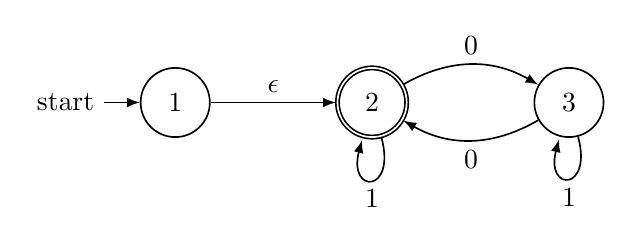
\begin{tikzpicture}[->,
            >=latex,
            auto,
            node distance=2.5cm,
            semithick,
            baseline=(top.base)]

        \node[initial,state]   (1)              {$1$};
        \node[accepting,state] (2) [right of=1] {$2$};
        \node[state]           (3) [right of=2] {$3$};

        \path (1) edge              node       {$\epsilon$} (2)
              (2) edge [loop below] node       {1}          (2)
                  edge [bend left]  node (top) {0}          (3)
              (3) edge [loop below] node       {1}          (3)
                  edge [bend left]  node       {0}          (2);
              
    \end{tikzpicture}
    \end{center}
    
    Now create \(N_{2}\) by swapping the accept and reject states of \(N_{1}\):
    \begin{center}       
    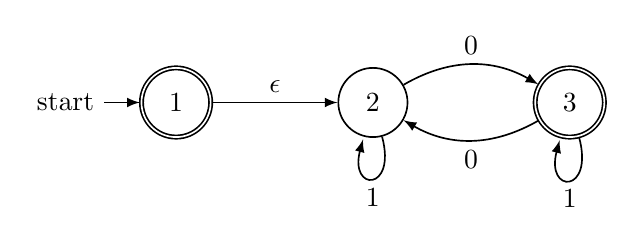
\begin{tikzpicture}[->,
            >=latex,
            auto,
            node distance=2.5cm,
            semithick,
            baseline=(top.base)]

        \node[initial,accepting,state] (1)              {$1$};
        \node[state]                   (2) [right of=1] {$2$};
        \node[accepting,state]         (3) [right of=2] {$3$};

        \path (1) edge              node       {$\epsilon$} (2)
              (2) edge [loop below] node       {1}          (2)
                  edge [bend left]  node (top) {0}          (3)
              (3) edge [loop below] node       {1}          (3)
                  edge [bend left]  node       {0}          (2);
              
    \end{tikzpicture}
    \end{center}
    
    Although this new NFA accepts strings with an odd number of 0s, it also accepts \(\epsilon\), and \(\epsilon \in L(N_{1})\), therefore \(L(N_{2}) \neq L(N_{1})^{\complement}\). This does not mean that the class of languages recognized by NFAs is not closed under complement. The class of languages recognized by NFAs is exactly the class of languages recognized by DFAs, and it was just shown that this class is closed under complement, therefore it is also true that the class of languages recognized by NFAs is closed under complement.
\end{enumerate}

\newpage
\addpoints
\question[25] Complete the five levels of Manufactoria (http://pleasingfungus.com/Manufactoria/) circled in red in the image below.
\begin{enumerate}
\item For each of your solutions, click the "Save" button (floppy disk icon), and copy the URL it gives you. (Note: Save is not available until after you complete level 1.)

\item Submit the URLs to your solutions on T-square.

\item Answer what does this game have to do with the material we study?\end{enumerate}
For clarity, the levels you will be submitting are:
\begin{itemize}
\item \textbf{Robotoast}! ACCEPT: Move robots from the entrance (top) to the exit (bottom)!
\item \textbf{Robocoffee}! If a robot's string starts with blue, accept. Otherwise, reject!
\item \textbf{Robolamp}! ACCEPT: if there are three or more blues!
\item \textbf{Robofish}! ACCEPT: if a robot contains NO red!
\item \textbf{Robobugs}! ACCEPT: if the tape has only alternating colors!
\end{itemize}
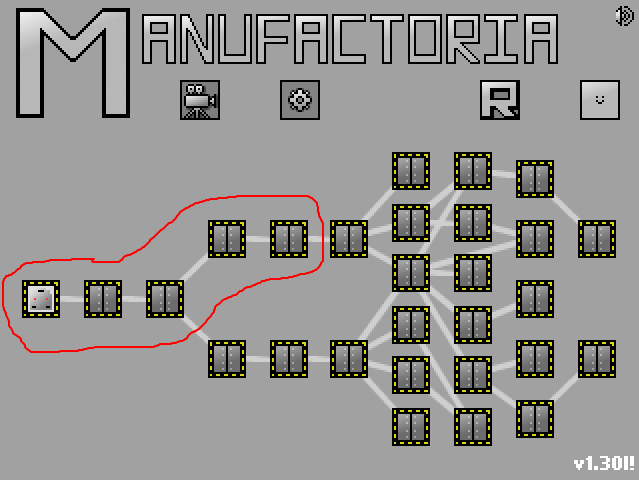
\includegraphics[scale=0.7]{manufactoria.png}

\subsection*{Answers}
This game basically simulates automata with the alphabet \(\{1,0\}\). The red and blue dots correspond to 0 and 1, and each robot's program corresponds to a string of that alphabet. The branches are like states in an automaton and the conveyors correspond to paths from one state to the next based on the input symbol.

\end{questions}

\end{document}
